% !TeX recipe = Rtex
% Optimizado para compilación rápida
\documentclass[paper=letter, fontsize=11pt, draft=false]{scrartcl}\usepackage[]{graphicx}\usepackage[]{xcolor}
% maxwidth is the original width if it is less than linewidth
% otherwise use linewidth (to make sure the graphics do not exceed the margin)
\makeatletter
\def\maxwidth{ %
  \ifdim\Gin@nat@width>\linewidth
    \linewidth
  \else
    \Gin@nat@width
  \fi
}
\makeatother

\definecolor{fgcolor}{rgb}{0.345, 0.345, 0.345}
\newcommand{\hlnum}[1]{\textcolor[rgb]{0.686,0.059,0.569}{#1}}%
\newcommand{\hlsng}[1]{\textcolor[rgb]{0.192,0.494,0.8}{#1}}%
\newcommand{\hlcom}[1]{\textcolor[rgb]{0.678,0.584,0.686}{\textit{#1}}}%
\newcommand{\hlopt}[1]{\textcolor[rgb]{0,0,0}{#1}}%
\newcommand{\hldef}[1]{\textcolor[rgb]{0.345,0.345,0.345}{#1}}%
\newcommand{\hlkwa}[1]{\textcolor[rgb]{0.161,0.373,0.58}{\textbf{#1}}}%
\newcommand{\hlkwb}[1]{\textcolor[rgb]{0.69,0.353,0.396}{#1}}%
\newcommand{\hlkwc}[1]{\textcolor[rgb]{0.333,0.667,0.333}{#1}}%
\newcommand{\hlkwd}[1]{\textcolor[rgb]{0.737,0.353,0.396}{\textbf{#1}}}%
\let\hlipl\hlkwb

\usepackage{framed}
\makeatletter
\newenvironment{kframe}{%
 \def\at@end@of@kframe{}%
 \ifinner\ifhmode%
  \def\at@end@of@kframe{\end{minipage}}%
  \begin{minipage}{\columnwidth}%
 \fi\fi%
 \def\FrameCommand##1{\hskip\@totalleftmargin \hskip-\fboxsep
 \colorbox{shadecolor}{##1}\hskip-\fboxsep
     % There is no \\@totalrightmargin, so:
     \hskip-\linewidth \hskip-\@totalleftmargin \hskip\columnwidth}%
 \MakeFramed {\advance\hsize-\width
   \@totalleftmargin\z@ \linewidth\hsize
   \@setminipage}}%
 {\par\unskip\endMakeFramed%
 \at@end@of@kframe}
\makeatother

\definecolor{shadecolor}{rgb}{.97, .97, .97}
\definecolor{messagecolor}{rgb}{0, 0, 0}
\definecolor{warningcolor}{rgb}{1, 0, 1}
\definecolor{errorcolor}{rgb}{1, 0, 0}
\newenvironment{knitrout}{}{} % an empty environment to be redefined in TeX

\usepackage{alltt}

% Modifications to layout
\usepackage[shortlabels]{enumitem} % Incisos

\newcommand{\RNum}[1]{\footnotesize\uppercase\expandafter{\romannumeral #1\relax\normalsize}} % Roman numbers

\usepackage{subcaption} % 2x2 graphs
\usepackage{mwe}

\usepackage{float} % [H] in graphics

\usepackage[hidelinks]{hyperref}  % Hipervínculos en la TOC


\usepackage{booktabs,siunitx,listings}
\usepackage[most]{tcolorbox}
\tcbuselibrary{theorems}
\usepackage{cleveref}

% Typography and layout packages
\usepackage{graphicx}
\usepackage{verbatim}
\usepackage{xcolor}
\usepackage[spanish,es-nodecimaldot]{babel} % Language and hyphenation
\usepackage{amsmath, amsfonts, amsthm, amssymb} % Math packages
\newtheorem{definition}{Definición} % definition
\newtheorem{theorem}{Teorema} % general theorem environment
\usepackage{fancyvrb}
\usepackage{sectsty} % Customize section commands
\usepackage{geometry} % Modify margins
\usepackage{titlesec} % Customize section titles
\geometry{margin=3cm,top=2.5cm,bottom=2.5cm} % Simplified geometry
\allsectionsfont{\centering \normalfont\scshape} % Center and style section titles

% Header and footer customization
\usepackage{fancyhdr}
\pagestyle{fancyplain}
\fancyhead[L]{\slshape} % Remove section title from header
\fancyhead[C]{} % Header center
\fancyhead[R]{\thepage} % Header right with page number
\fancyfoot[L]{} % Footer left
\fancyfoot[C]{} % Footer center
\fancyfoot[R]{\small \slshape Gustavo Hernández Angeles} % Footer right
\renewcommand{\headrulewidth}{0.4pt} % Header rule
\renewcommand{\footrulewidth}{0.4pt} % Footer rule
\setlength{\headheight}{14.5pt} % Header height



% Paragraph settings
\setlength\parindent{0pt}
\setlength{\parskip}{1ex}

% Section spacing
\titlespacing*{\section}{0cm}{0.50cm}{0.25cm}

% --- Theorems, lemma, corollary, postulate, definition ---
\definecolor{Pantone209C}{HTML}{64293e}

\newcounter{problemcounter}

\numberwithin{equation}{problemcounter} % Number equations within problems
\numberwithin{figure}{problemcounter} % Number figures within problems
\numberwithin{table}{problemcounter} % Number tables within problems
\numberwithin{subsection}{problemcounter} 

\newtcbtheorem[auto counter]{problem}{Ejercicio}{
    enhanced,
    breakable,
    colback = gray!5,
    colframe = gray!5,
    boxrule = 0.5pt,
    sharp corners,
    borderline west = {2mm}{0mm}{Pantone209C},
    fonttitle = \bfseries\sffamily,
    coltitle = Pantone209C,
    drop fuzzy shadow,
    parbox = false,
    before skip = 3ex,
    after skip = 3ex
}{problem}
\makeatletter
\renewenvironment{problem}[2][]{%
    \refstepcounter{problemcounter}%
    \addcontentsline{toc}{section}{\protect\numberline{\theproblemcounter}Ejercicio \theproblemcounter: #2}%
    \begin{tcolorbox}[
        enhanced,
        breakable,
        colback = gray!5,
        colframe = gray!5,
        boxrule = 0.5pt,
        sharp corners,
        borderline west = {2mm}{0mm}{Pantone209C},
        fonttitle = \bfseries\sffamily,
        coltitle = Pantone209C,
        drop fuzzy shadow,
        parbox = false,
        before skip = 3ex,
        after skip = 3ex,
        title={Ejercicio \theproblemcounter: #2}
    ]
}{%
    \end{tcolorbox}
}
\makeatother




\tcbuselibrary{skins, breakable}
% Custom command for a horizontal rule
\newcommand{\horrule}[1]{\rule{\linewidth}{#1}} 

% Custom section titles
\titleformat{\section}
{\normalfont\Large\bfseries}{}{1em}{}

\titleformat{\subsection}
{\normalfont\large\bfseries}{}{1em}{}

\titleformat{\subsubsection}
{\normalfont\normalsize\bfseries}{\thesubsubsection}{1em}{}

% Title and author
\title{	
    \begin{center}
        
\includegraphics[width=3cm]{figure/template/cimat-logo.png} % Adjust size as needed
    \end{center}
    \vspace{0.5cm}
    \normalfont \normalsize 
    \textbf{\Large   Centro de Investigación en Matemáticas} \\
    \Large Unidad Monterrey \\ [25pt] 
    \horrule{1pt} \\[0.4cm] % Thin top horizontal rule
    \huge Cómputo Estadístico\\
    \huge Tarea 3: MCMC y Bootstrap \\ 
    \horrule{2pt} \\[0.5cm] % Thick bottom horizontal rule
}

\author{\large Gustavo Hern\'andez Angeles}    

\date{\normalsize\today} % Today's date
\IfFileExists{upquote.sty}{\usepackage{upquote}}{}
\begin{document}




















%%%%%%%%%%% PROBLEMA 1 %%%%%%%%%%%
% TEMA: Prueba de hipótesis para una media, varianza conocida (Diapositivas 38-46)
\begin{problem}{}
    Un fabricante de cables de acero afirma que la resistencia media a la ruptura de sus cables es de $\mu = 5000$ kg. Se sabe por experiencia histórica que la desviación estándar de la resistencia a la ruptura es $\sigma = 200$ kg. Un ingeniero de control de calidad sospecha que la resistencia media ha cambiado (ya sea aumentado o disminuido). Para verificarlo, selecciona una muestra aleatoria de $n = 25$ cables y obtiene una media muestral de $\bar{x} = 4920$ kg. Realice una prueba de hipótesis con un nivel de significancia $\alpha = 0.05$.
\end{problem}

\subsection{\textbf{Solución:}}

Queremos probar si la media es diferente del valor histórico.
$$H_0: \mu = 5000$$
$$H_1: \mu \neq 5000$$

A un nivel de significancia de
$\alpha = 0.05$.


Dado que la varianza poblacional $\sigma^2$ es conocida y, \textbf{asumiendo} que la distribución de la resistencia es normal (o \textbf{aplicamos} el Teorema del Límite Central), utilizamos el estadístico $Z$:
$$Z = \frac{\bar{X} - \mu_0}{\sigma / \sqrt{n}}$$

Sustituyendo los valores:
$$Z = \frac{4920 - 5000}{200 / \sqrt{25}} = \frac{-80}{200 / 5} = \frac{-80}{40} = -2.0$$

Para una prueba bilateral con $\alpha = 0.05$, la masa de probabilidad se reparte en ambas colas ($\alpha/2 = 0.025$). Los valores críticos son $Z_{0.025} = \pm 1.96$.
La región de rechazo es $R = \{z \mid z < -1.96 \text{ ó } z > 1.96\}$.

\begin{figure}[H]
    \centering
    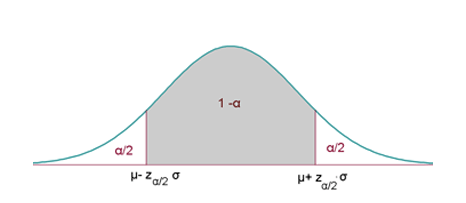
\includegraphics[width=0.6\textwidth]{figure/bilateral.png}
    \caption{Región de rechazo para la prueba bilateral.}
\end{figure}

Como el estadístico calculado $Z = -2.0$ cae dentro de la región de rechazo ($ -2.0 < -1.96$), \textbf{rechazamos la hipótesis nula $H_0$}. Existe evidencia estadística suficiente al 5\% de significancia para afirmar que la resistencia media de los cables es diferente de 5000 kg.

\newpage

%%%%%%%%%%% PROBLEMA 2 %%%%%%%%%%%
% TEMA: Prueba de hipótesis para una media, varianza desconocida (Diapositiva 66 - análogo t-student una muestra)
\begin{problem}{}
    Una organización de consumidores afirma que el tiempo medio de vida de una batería específica es a lo sumo de 40 horas. El fabricante sostiene que es mayor. Se toma una muestra aleatoria de $n = 16$ baterías, obteniendo una media muestral $\bar{x} = 42.5$ horas y una varianza muestral $s^2 = 16$. Asuma que la vida de las baterías sigue una distribución normal. Pruebe la afirmación del fabricante con un nivel de significancia $\alpha = 0.01$.
\end{problem}

\subsection{\textbf{Solución:}}

El fabricante quiere probar que la media es mayor a 40 (hipótesis de investigación en $H_1$).
$$H_0: \mu \leq 40$$
$$H_1: \mu > 40$$

A un nivel de significancia de
$\alpha = 0.01$.

Como la varianza poblacional es desconocida y el tamaño de muestra es pequeño ($n < 30$), utilizamos el estadístico $t$ de Student con $n-1$ grados de libertad:
$$t = \frac{\bar{X} - \mu_0}{S / \sqrt{n}}$$
Donde $S = \sqrt{16} = 4$.
$$t = \frac{42.5 - 40}{4 / \sqrt{16}} = \frac{2.5}{4 / 4} = 2.5$$


Es una prueba unilateral derecha. Buscamos el valor crítico $t_{\alpha, n-1} = t_{0.01, 15}$.
Consultando la tabla de la distribución $t$, $t_{0.01, 15} = 2.602$.
La región de rechazo es $R = \{t \mid t > 2.602\}$.

El estadístico calculado $t = 2.5$ no es mayor que el valor crítico $2.602$. Por lo tanto, \textbf{no rechazamos la hipótesis nula $H_0$}. A un nivel de significancia del 1\%, no hay evidencia suficiente para respaldar la afirmación del fabricante de que la vida media es superior a 40 horas.

\newpage

%%%%%%%%%%% PROBLEMA 3 %%%%%%%%%%%
% TEMA: Comparación de dos poblaciones, varianzas conocidas (Diapositivas 57-59)
\begin{problem}{}
    Se comparan dos métodos de enseñanza (A y B) para determinar si el Método A produce calificaciones promedio superiores. Se asume que las varianzas de las calificaciones poblacionales son conocidas: $\sigma_A^2 = 50$ y $\sigma_B^2 = 40$. Se toman muestras independientes con los siguientes resultados:
    \begin{itemize}
        \item Método A: $n_A = 75$, $\bar{x}_A = 88$.
        \item Método B: $n_B = 60$, $\bar{x}_B = 85$.
    \end{itemize}
    Pruebe la hipótesis de que $\mu_A > \mu_B$ usando $\alpha = 0.05$. Calcule también el p-valor.
\end{problem}

\subsection{\textbf{Solución:}}

\textbf{Probando la hipotesis}

Se plantean las hipótesis:
$$H_0: \mu_A \leq \mu_B \quad (\text{o } \mu_A - \mu_B \leq 0)$$
$$H_1: \mu_A > \mu_B \quad (\text{o } \mu_A - \mu_B > 0)$$

Con varianzas conocidas y muestras independientes, el estadístico es:
$$Z = \frac{(\bar{X}_A - \bar{X}_B) - (\mu_A - \mu_B)}{\sqrt{\frac{\sigma_A^2}{n_A} + \frac{\sigma_B^2}{n_B}}}$$
Bajo $H_0$ en el límite, $(\mu_A - \mu_B) = 0$.
$$Z = \frac{88 - 85}{\sqrt{\frac{50}{75} + \frac{40}{60}}} = \frac{3}{\sqrt{0.6667 + 0.6667}} = \frac{3}{\sqrt{1.3334}} \approx \frac{3}{1.1547} \approx 2.598$$

Para $\alpha = 0.05$ (cola derecha), el valor crítico es $Z_{0.05} = 1.645$.
Región de rechazo: $Z > 1.645$.

\textbf{Calculamos el p-valor}

Calculamos el p-valor:
$$p\text{-valor} = P(Z > 2.598) = 1 - P(Z \leq 2.598)$$
Usando tablas normales, $P(Z \leq 2.60) \approx 0.9953$.
$$p\text{-valor} \approx 1 - 0.9953 = 0.0047$$


Como $Z_{calc} = 2.598 > 1.645$ (y el p-valor $0.0047 < 0.05$), \textbf{rechazamos $H_0$}. Se concluye que el promedio de calificaciones del Método A es significativamente mayor que el del Método B.

\newpage

%%%%%%%%%%% PROBLEMA 4 %%%%%%%%%%%
% TEMA: Comparación de dos poblaciones, varianzas desconocidas pero iguales (Pooled) (Diapositivas 61-65)
\begin{problem}{}
    Se lleva a cabo un estudio para comparar el contenido de nicotina de dos marcas de cigarrillos. Se asume que las poblaciones son normales y tienen varianzas iguales ($\sigma_1^2 = \sigma_2^2$), aunque desconocidas.
    \begin{itemize}
        \item Marca 1: $n_1 = 10$, $\bar{x}_1 = 18.5$ mg, $s_1^2 = 2.5$.
        \item Marca 2: $n_2 = 12$, $\bar{x}_2 = 20.1$ mg, $s_2^2 = 3.2$.
    \end{itemize}
    Determine si existe una diferencia significativa entre los contenidos medios de nicotina con $\alpha = 0.05$.
\end{problem}

\subsection{\textbf{Solución:}}

Establecemos las hipotesis nula y alternativa:
$$H_0: \mu_1 = \mu_2$$
$$H_1: \mu_1 \neq \mu_2$$


Debemos calcular la varianza ponderada:
$$S_p^2 = \frac{(n_1 - 1)S_1^2 + (n_2 - 1)S_2^2}{n_1 + n_2 - 2}$$
$$S_p^2 = \frac{(9)(2.5) + (11)(3.2)}{10 + 12 - 2} = \frac{22.5 + 35.2}{20} = \frac{57.7}{20} = 2.885$$
La desviación estándar agrupada es $S_p = \sqrt{2.885} \approx 1.6985$.


Utilizamos el estadístico $t$ para varianzas iguales:
$$t = \frac{(\bar{X}_1 - \bar{X}_2)}{S_p \sqrt{\frac{1}{n_1} + \frac{1}{n_2}}}$$
$$t = \frac{18.5 - 20.1}{1.6985 \sqrt{\frac{1}{10} + \frac{1}{12}}} = \frac{-1.6}{1.6985 \sqrt{0.1 + 0.0833}} = \frac{-1.6}{1.6985 \sqrt{0.1833}}$$
$$t = \frac{-1.6}{1.6985 (0.4281)} = \frac{-1.6}{0.7271} \approx -2.20$$


Los grados de libertad se calculan como $v = n_1 + n_2 - 2 = 20$.
Para una prueba bilateral con $\alpha = 0.05$, buscamos $t_{\alpha/2, v} = t_{0.025, 20}$.
En tablas, $t_{0.025, 20} = 2.086$.
La región de rechazo es $|t| > 2.086$ (es decir, $t < -2.086$ o $t > 2.086$).

Dado que el estadístico calculado $t = -2.20$ cae en la región de rechazo ($ -2.20 < -2.086$), \textbf{rechazamos $H_0$}. Existe evidencia suficiente para afirmar que hay una diferencia significativa en el contenido medio de nicotina entre ambas marcas.

\newpage


% \nocite{*}
% \bibliographystyle{plainnat} % Elige un estilo (otros: abbrvnat, unsrtnat, etc.)
% \bibliography{bib} % Indica el nombre de tu archivo .bib (sin la extensión)

\end{document}
                                                                                                                                                                                                                                                                                                                                                        
